\documentclass[11pt, oneside]{article}   	% use "amsart" instead of "article" for AMSLaTeX format
\usepackage{geometry}                		% See geometry.pdf to learn the layout options. There are lots.
\geometry{letterpaper}                   		% ... or a4paper or a5paper or ... 
\usepackage[pdftex]{graphicx} % For including graphics N.B. pdftex graphics driver 	
\usepackage{amssymb}
\usepackage{amsmath}
\usepackage{centernot}
\usepackage{enumerate}
\usepackage{graphicx}

\setlength{\marginparwidth}{0pt} % width of margin notes
% N.B. If margin notes are used, you must adjust \textwidth, \marginparwidth
% and \marginparsep so that the space left between the margin notes and page
% edge is less than 15 mm (0.6 in.)
\setlength{\marginparsep}{0pt} % width of space between body text and margin notes
\setlength{\evensidemargin}{0.125in} % Adds 1/8 in. to binding side of all 
% even-numbered pages when the "twoside" printing option is selected
\setlength{\oddsidemargin}{0.125in} % Adds 1/8 in. to the left of all pages
% when "oneside" printing is selected, and to the left of all odd-numbered
% pages when "twoside" printing is selected
\setlength{\textwidth}{6.375in} % assuming US letter paper (8.5 in. x 11 in.) and 
% side margins as above
\raggedbottom


\title{CS348 - Databases, A04}
\author{Edward Yang, 20378808}
%\date{}							% Activate to display a given date or no date

\begin{document}
\maketitle
\begin{enumerate}
\item 
\begin{verbatim}
create table PERSON
(
  LICENSE# int NOT NULL,
  DATE_OF_BIRTH date NOT NULL,
  NAME varchar(255) NOT NULL,
  PRIMARY KEY (LICENSE#)
);

create table CAR
(
  VIN# int NOT NULL,
  MODEL varchar(255) NOT NULL,
  YEAR int NOT NULL,
  PRIMARY KEY (VIN#)
);

create table OWN
(
  LICENSE# int NOT NULL,
  VIN# int NOT NULL,
  FROM date NOT NULL,
  UNTIL date NOT NULL,
  foreign key (LICENSE#) references PERSON (LICENSE#),
  foreign key (VIN#) references CAR (LICENSE#),

  constraint uniqueVIN UNIQUE (VIN#), // ensures car is only owned by one person
  constraint limitLICENSE CHECK (LICENSE# <= 10 AND LICENSE# >= 0)
);
\end{verbatim}
\item $R = \{X, Q, Z, L, T, U\}$, $X = \{X, L\}$, $F = F$
\begin{enumerate}[(a)]
\item Using Schema Refinement - Slide 17
\\ $X^+ = \{X, L\}$
\\ $X^+ = \{X, L, Q\}$ ($X \rightarrow Q$)
\\ $X^+ = \{X, L, Q, Z\}$ ($X \rightarrow Z$)
\\ $X^+ = \{X, L, Q, Z, T\}$ ($ZL \rightarrow T$)
\\ $X^+ = \{X, L, Q, Z, T, U\}$ ($ZL \rightarrow U$)
\\ end loop
\item Yes, XL is a candidate key since $X^+ \supseteq R$.
\end{enumerate}
\item $R = R$, $F = F$
\\ We know that it is lossless if and only if common attributes of R1 and R2 form a superkey.
\\ i.e. $R1 \cap R2 \rightarrow R1$ or $R1 \cap R2 \rightarrow R2$
\\ \\ $R1 \cap R2 = \{V\}$
\\ Let $X^+ = \{V\}$
\\ $X^+ = \{V, W, X\}$ ($V \rightarrow WX$)
\\ $X^+ = \{V, W, X, Y\}$ ($W \rightarrow Y$)
\\ $X^+ = \{V, W, X, Y, Z\}$ ($XY \rightarrow Z$)
\\ end loop
\\ $\implies \{V\}$ is a candidate key, it is also a (minimal) superkey.
\\ Since $\{V\}$ is the common attribute of R1, R2 and form a superkey. 
\\ $\implies$ this decomposition is lossless.
\\ Q.E.D.
\item
\begin{enumerate}[(a)]
\item q: $(r_1, w_3), (w_1, w_3), (w_1, r_2), (w_3, r_2)$
\\ x: $(w_1, r_2), (w_1, r_5)$
\\ y: $(w_4, r_2), (r_2, w_5)$
\\ z: $(r_3, w_4), (w_3, w_4) $
\item
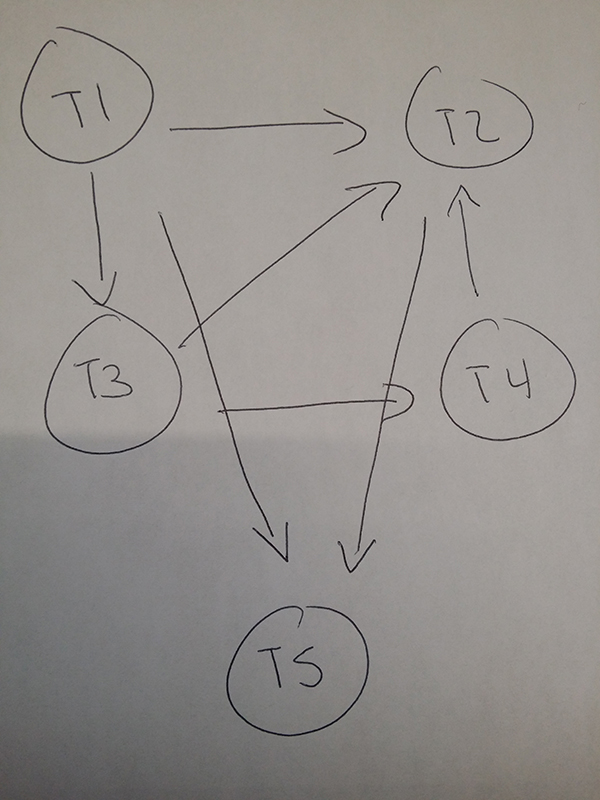
\includegraphics[scale=0.2]{graph1.jpg}
\item This schedule is serializable as T1, T3, T4, T2, T5
\\ $r_1(q)\ w_1(x)\ w_1(q)\ r_3(z)\ w_3(z)\ w_3(q)\ w_4(y)\ w_4(z)\ r_2(y)\ r_2(x)\ r_2(q)\ r_5(x)\ w_5(y)$
\end{enumerate}
\item
\begin{enumerate}[(a)]
\item $T_2$: write x, $T_2$: read y, $T_4$: write z, $T_2$: commit, $T_5$: write z, $T_4$: abort
\item No. 
\item Yes, this execution order is serializable. Any order of (T1, T3) followed by any order of (T2, T4, T5). Eg. T1, T3, T2, T4, T5
\\ Example execution order:
\\ 1. $T_1$: read x - gets shared lock on x
\\ 2. $T_3$: read x - gets shared lock on x
\\ 3. $T_2$: write x - [BLOCK] tries to acquire exclusive lock on x
\\ 4. $T_2$: read y - doesn't run until above
\\ 5. $T_1$: read y - gets shared lock on y
\\ 6. $T_3$: read z - gets shared lock on z
\\ 7. $T_1$: commit - releases shared lock on x. 3 still blocked because $T_3$ holds shared lock
\\ 8. $T_4$: write z - [BLOCK] tries to acquire exclusive lock on z
\\ 9. $T_2$: commit - doesn't run until 3.
\\ 10. $T_5$: write z - [BLOCK] tries on acquire exlusive lock on z
\\ 11. $T_4$: abort - doesn't run until 8.
\\ 12. $T_3$: commit - releases shared lock on x, z
\\ 13. (line 3 runs) - acquires exclusive lock on x
\\ 14. (line 4 runs) - acquires shared lock on y
\\ 15. (line 9 runs) - releases locks on x, y
\\ 16. (line 8 runs) - acquires exclusive lock on z
\\ 17. (line 11 runs) - releases lock on z
\\ 18. (line 10 runs) - acquires exclusive lock on z
\\ 19. $T_5$: commit - releases exclusive lock on z
\end{enumerate}
\item
\begin{enumerate}[(a)]
\item You would require 50 disk accesses - you need to retrieve all 1000 students and you get 20 records per disk access = $(1000/20)$
\item c - The algorithm will go down as deep as necessary before it notices that the left and right records are the same at which point it will stop descending down that path.
\end{enumerate}
\item
What database system must do:
\\1. Go through log and create a list of transactions (committed, active, aborted) in order
\\2. Undo active/aborted (newest to oldest)
\\3. Redo committed (oldest to newest)
\\ 
\\Committed: T1, T3, T5, Active: T2, T6, Aborted: T4
\\
\\ objects that need to be modified A, X, Y, Z
\\ order of modifications (from top to bottom)
\\ A= 2 - Undo (T6, A, 2, 3)
\\ X = 400 - Undo (T6, X, 400, 0)
\\ A = 0 - Undo (T4, A, 0, 1)
\\ Y = 10 - Undo (T2, Y, 10, 20)
\\ X = 10 - (T1, X, 0, 10)
\\ X = 400 - (T3, X, 10, 400)
\\ Z= 100 - (T3, Z, 0, 100)
\\ A = 2 - (T5, A, 0, 2) 
\\
\\ After failure recovery: T1, T3, T5 are committed and T2, T4, T6 are aborted.
\end{enumerate}
%\section{}
%\subsection{}



\end{document}  